\documentclass{standalone}
\usepackage{tikz}
\usetikzlibrary{patterns}
\usetikzlibrary{positioning}
\usetikzlibrary{patterns, positioning}
\usetikzlibrary{shapes.misc}
\usepackage[outline]{contour}
\contourlength{1.5pt} 
\usetikzlibrary{calc}
        \usepackage{relsize}
        \tikzset{fontscale/.style = {font=\relsize{#1}}}

\begin{document}
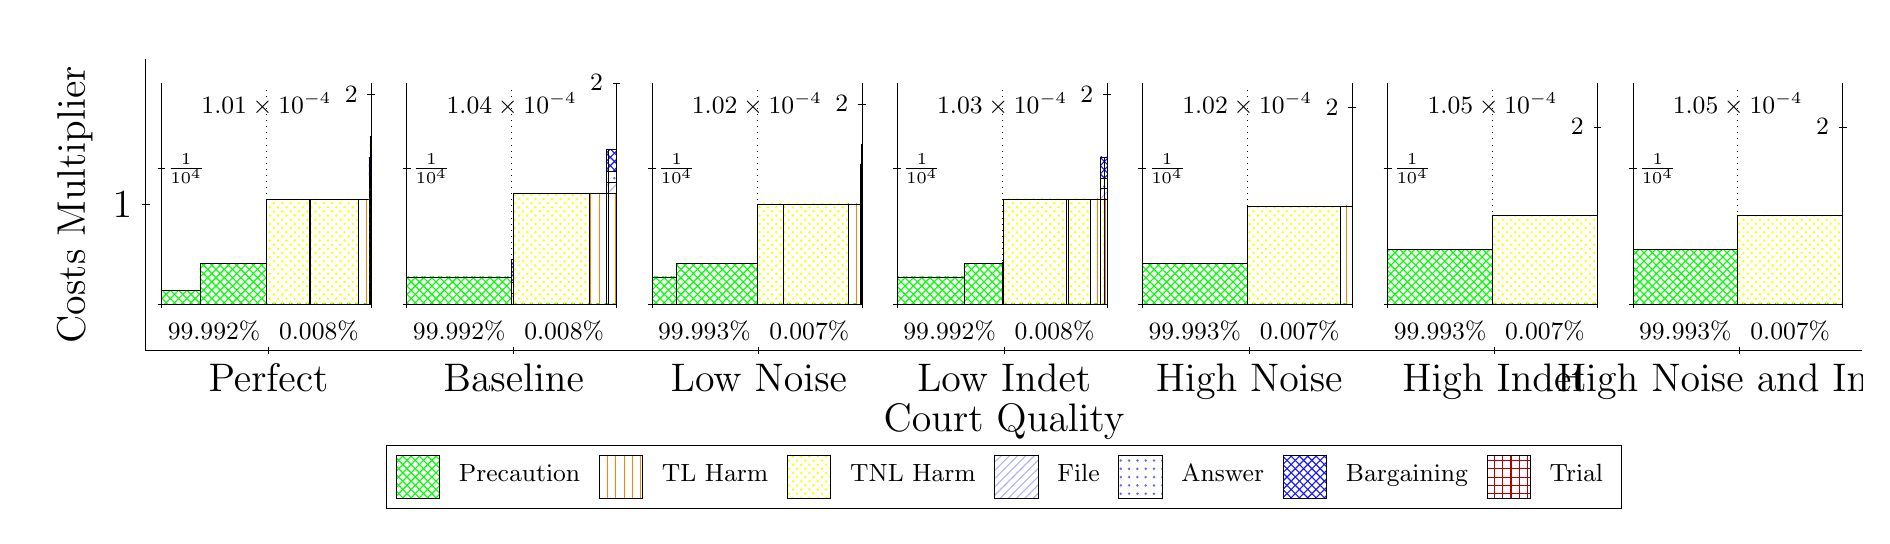
\begin{tikzpicture}
\clip(-0.5,-1.1) rectangle +(23.3,6.2);
\draw[black] (1,1) -- (1,4.7);
\node[rotate=90, fontscale=2, anchor=center] at (0.1, 2.85) {Costs Multiplier};
\draw[black] (0.95,2.85) -- (1.05,2.85);
\node[fontscale=2, anchor=east] at (0.95, 2.85) {1};

\draw[black] (1,1) -- (22.8,1);
\node[fontscale=2, anchor=center] at (11.9, 0.1) {Court Quality};
\draw[black] (2.5571,0.95) -- (2.5571,1.05);
\node[fontscale=2, anchor=north] at (2.5571, 0.95) {Perfect};
\draw[black] (5.6714,0.95) -- (5.6714,1.05);
\node[fontscale=2, anchor=north] at (5.6714, 0.95) {Baseline};
\draw[black] (8.7857,0.95) -- (8.7857,1.05);
\node[fontscale=2, anchor=north] at (8.7857, 0.95) {Low Noise};
\draw[black] (11.9,0.95) -- (11.9,1.05);
\node[fontscale=2, anchor=north] at (11.9, 0.95) {Low Indet};
\draw[black] (15.014,0.95) -- (15.014,1.05);
\node[fontscale=2, anchor=north] at (15.014, 0.95) {High Noise};
\draw[black] (18.129,0.95) -- (18.129,1.05);
\node[fontscale=2, anchor=north] at (18.129, 0.95) {High Indet};
\draw[black] (21.243,0.95) -- (21.243,1.05);
\node[fontscale=2, anchor=north] at (21.243, 0.95) {High Noise and Indet};


\draw[pattern=crosshatch, pattern color=green,draw=black,very thin] (1.2,1.592) rectangle (1.6864,1.764);
\draw[pattern=crosshatch, pattern color=green,draw=black,very thin] (1.6864,1.592) rectangle (2.5321,2.1081);
\draw[pattern=crosshatch, pattern color=green,draw=black,very thin] (2.5321,1.592) rectangle (2.5336,1.592);
\draw[pattern=north east lines, pattern color=blue!30,draw=black,very thin] (2.5321,1.592) rectangle (2.5336,1.7251);
\draw[pattern=dots,  pattern color=blue!60,draw=black,very thin] (2.5321,1.7251) rectangle (2.5336,1.8582);
\draw[pattern=crosshatch,      pattern color=blue!90,draw=black,very thin] (2.5321,1.8582) rectangle (2.5336,2.1245);
\draw[pattern=crosshatch, pattern color=green,draw=black,very thin] (2.5336,1.592) rectangle (2.5355,1.592);
\draw[pattern=north east lines, pattern color=blue!30,draw=black,very thin] (2.5336,1.592) rectangle (2.5355,1.7251);
\draw[pattern=dots,  pattern color=blue!60,draw=black,very thin] (2.5336,1.7251) rectangle (2.5355,1.8582);
\draw[pattern=crosshatch,      pattern color=blue!90,draw=black,very thin] (2.5336,1.8582) rectangle (2.5355,2.1245);
\draw[pattern=grid,            pattern color=red!70!black,draw=black,very thin] (2.5336,2.1245) rectangle (2.5355,2.3907);
\draw[pattern=crosshatch, pattern color=green,draw=black,very thin] (2.5355,1.592) rectangle (3.0765,1.592);
\draw[pattern=crosshatch dots, pattern color=yellow,draw=black,very thin] (2.5355,1.592) rectangle (3.0765,2.9232);
\draw[pattern=crosshatch, pattern color=green,draw=black,very thin] (3.0765,1.592) rectangle (3.0843,1.592);
\draw[pattern=vertical lines, pattern color=orange,draw=black,very thin] (3.0765,1.592) rectangle (3.0843,2.9232);
\draw[pattern=crosshatch, pattern color=green,draw=black,very thin] (3.0843,1.592) rectangle (3.7014,1.592);
\draw[pattern=crosshatch dots, pattern color=yellow,draw=black,very thin] (3.0843,1.592) rectangle (3.7014,2.9232);
\draw[pattern=crosshatch, pattern color=green,draw=black,very thin] (3.7014,1.592) rectangle (3.8342,1.592);
\draw[pattern=vertical lines, pattern color=orange,draw=black,very thin] (3.7014,1.592) rectangle (3.8342,2.9232);
\draw[pattern=crosshatch, pattern color=green,draw=black,very thin] (3.8342,1.592) rectangle (3.8452,1.592);
\draw[pattern=crosshatch dots, pattern color=yellow,draw=black,very thin] (3.8342,1.592) rectangle (3.8452,2.9232);
\draw[pattern=north east lines, pattern color=blue!30,draw=black,very thin] (3.8342,2.9232) rectangle (3.8452,3.0563);
\draw[pattern=dots,  pattern color=blue!60,draw=black,very thin] (3.8342,3.0563) rectangle (3.8452,3.1894);
\draw[pattern=crosshatch,      pattern color=blue!90,draw=black,very thin] (3.8342,3.1894) rectangle (3.8452,3.4556);
\draw[pattern=crosshatch, pattern color=green,draw=black,very thin] (3.8452,1.592) rectangle (3.8474,1.592);
\draw[pattern=vertical lines, pattern color=orange,draw=black,very thin] (3.8452,1.592) rectangle (3.8474,2.9232);
\draw[pattern=north east lines, pattern color=blue!30,draw=black,very thin] (3.8452,2.9232) rectangle (3.8474,3.0563);
\draw[pattern=dots,  pattern color=blue!60,draw=black,very thin] (3.8452,3.0563) rectangle (3.8474,3.1894);
\draw[pattern=crosshatch,      pattern color=blue!90,draw=black,very thin] (3.8452,3.1894) rectangle (3.8474,3.4556);
\draw[pattern=crosshatch, pattern color=green,draw=black,very thin] (3.8474,1.592) rectangle (3.8584,1.592);
\draw[pattern=crosshatch dots, pattern color=yellow,draw=black,very thin] (3.8474,1.592) rectangle (3.8584,2.9232);
\draw[pattern=north east lines, pattern color=blue!30,draw=black,very thin] (3.8474,2.9232) rectangle (3.8584,3.0563);
\draw[pattern=dots,  pattern color=blue!60,draw=black,very thin] (3.8474,3.0563) rectangle (3.8584,3.1894);
\draw[pattern=crosshatch,      pattern color=blue!90,draw=black,very thin] (3.8474,3.1894) rectangle (3.8584,3.4556);
\draw[pattern=grid,            pattern color=red!70!black,draw=black,very thin] (3.8474,3.4556) rectangle (3.8584,3.7219);
\draw[pattern=crosshatch, pattern color=green,draw=black,very thin] (3.8584,1.592) rectangle (3.8643,1.592);
\draw[pattern=vertical lines, pattern color=orange,draw=black,very thin] (3.8584,1.592) rectangle (3.8643,2.9232);
\draw[pattern=north east lines, pattern color=blue!30,draw=black,very thin] (3.8584,2.9232) rectangle (3.8643,3.0563);
\draw[pattern=dots,  pattern color=blue!60,draw=black,very thin] (3.8584,3.0563) rectangle (3.8643,3.1894);
\draw[pattern=crosshatch,      pattern color=blue!90,draw=black,very thin] (3.8584,3.1894) rectangle (3.8643,3.4556);
\draw[pattern=grid,            pattern color=red!70!black,draw=black,very thin] (3.8584,3.4556) rectangle (3.8643,3.7219);
\node[font=\small,text=black,anchor=north] at (2.5321, 4.4) {$1.01\times 10^{-4}$};
\draw[black,very thin] (1.2,1.592) -- (1.2,4.4);
\draw[black,very thin] (1.15,1.592) -- (1.25,1.592);
\node[font=\small,text=black, anchor=west] at (1.15, 1.592) {};
\draw[black,very thin] (1.15,3.3123) -- (1.25,3.3123);
\node[font=\small,text=black, anchor=west] at (1.15, 3.3123) {$\frac{1}{10^{4}}$};

\draw[black,dotted,very thin] (2.5321,1.6762) -- (2.5321,4.3158);
\draw[black,very thin] (3.8643,1.592) -- (3.8643,4.4);
\draw[black,very thin] (3.8143,4.2543) -- (3.9143,4.2543);
\node[font=\small,text=black, anchor=east] at (3.8143, 4.2543) {\contour{white}{2}};

\draw[black,very thin] (1.2,1.592) -- (3.8643,1.592);
\draw[black,very thin] (1.2,1.542) -- (1.2,1.642);
\node[font=\small,text=black, anchor=north] at (1.2, 1.542) {};
\draw[black,very thin] (3.8643,1.542) -- (3.8643,1.642);
\node[font=\small,text=black, anchor=north] at (3.8643, 1.542) {};

\node[font=\small,text=black,anchor=south] at (1.8661, 0.992) {99.992\%};
\node[font=\small,text=black,anchor=south] at (3.1982, 0.992) {0.008\%};

\draw[pattern=crosshatch, pattern color=green,draw=black,very thin] (4.3143,1.592) rectangle (5.6464,1.9361);
\draw[pattern=crosshatch, pattern color=green,draw=black,very thin] (5.6464,1.592) rectangle (5.6632,1.592);
\draw[pattern=north east lines, pattern color=blue!30,draw=black,very thin] (5.6464,1.592) rectangle (5.6632,1.7324);
\draw[pattern=dots,  pattern color=blue!60,draw=black,very thin] (5.6464,1.7324) rectangle (5.6632,1.8728);
\draw[pattern=crosshatch,      pattern color=blue!90,draw=black,very thin] (5.6464,1.8728) rectangle (5.6632,2.1536);
\draw[pattern=crosshatch, pattern color=green,draw=black,very thin] (5.6632,1.592) rectangle (6.6343,1.592);
\draw[pattern=crosshatch dots, pattern color=yellow,draw=black,very thin] (5.6632,1.592) rectangle (6.6343,2.996);
\draw[pattern=crosshatch, pattern color=green,draw=black,very thin] (6.6343,1.592) rectangle (6.8526,1.592);
\draw[pattern=vertical lines, pattern color=orange,draw=black,very thin] (6.6343,1.592) rectangle (6.8526,2.996);
\draw[pattern=crosshatch, pattern color=green,draw=black,very thin] (6.8526,1.592) rectangle (6.8765,1.592);
\draw[pattern=crosshatch dots, pattern color=yellow,draw=black,very thin] (6.8526,1.592) rectangle (6.8765,2.996);
\draw[pattern=north east lines, pattern color=blue!30,draw=black,very thin] (6.8526,2.996) rectangle (6.8765,3.1364);
\draw[pattern=dots,  pattern color=blue!60,draw=black,very thin] (6.8526,3.1364) rectangle (6.8765,3.2768);
\draw[pattern=crosshatch,      pattern color=blue!90,draw=black,very thin] (6.8526,3.2768) rectangle (6.8765,3.5576);
\draw[pattern=crosshatch, pattern color=green,draw=black,very thin] (6.8765,1.592) rectangle (6.9783,1.592);
\draw[pattern=vertical lines, pattern color=orange,draw=black,very thin] (6.8765,1.592) rectangle (6.9783,2.996);
\draw[pattern=north east lines, pattern color=blue!30,draw=black,very thin] (6.8765,2.996) rectangle (6.9783,3.1364);
\draw[pattern=dots,  pattern color=blue!60,draw=black,very thin] (6.8765,3.1364) rectangle (6.9783,3.2768);
\draw[pattern=crosshatch,      pattern color=blue!90,draw=black,very thin] (6.8765,3.2768) rectangle (6.9783,3.5576);
\draw[pattern=crosshatch, pattern color=green,draw=black,very thin] (6.9783,1.592) rectangle (6.9786,1.592);
\draw[pattern=crosshatch dots, pattern color=yellow,draw=black,very thin] (6.9783,1.592) rectangle (6.9786,2.996);
\draw[pattern=north east lines, pattern color=blue!30,draw=black,very thin] (6.9783,2.996) rectangle (6.9786,3.1364);
\draw[pattern=dots,  pattern color=blue!60,draw=black,very thin] (6.9783,3.1364) rectangle (6.9786,3.2768);
\draw[pattern=crosshatch,      pattern color=blue!90,draw=black,very thin] (6.9783,3.2768) rectangle (6.9786,3.5576);
\draw[pattern=grid,            pattern color=red!70!black,draw=black,very thin] (6.9783,3.5576) rectangle (6.9786,3.8384);
\node[font=\small,text=black,anchor=north] at (5.6464, 4.4) {$1.04\times 10^{-4}$};
\draw[black,very thin] (4.3143,1.592) -- (4.3143,4.4);
\draw[black,very thin] (4.2643,1.592) -- (4.3643,1.592);
\node[font=\small,text=black, anchor=west] at (4.2643, 1.592) {};
\draw[black,very thin] (4.2643,3.3123) -- (4.3643,3.3123);
\node[font=\small,text=black, anchor=west] at (4.2643, 3.3123) {$\frac{1}{10^{4}}$};

\draw[black,dotted,very thin] (5.6464,1.6762) -- (5.6464,4.3158);
\draw[black,very thin] (6.9786,1.592) -- (6.9786,4.4);
\draw[black,very thin] (6.9286,4.4) -- (7.0286,4.4);
\node[font=\small,text=black, anchor=east] at (6.9286, 4.4) {\contour{white}{2}};

\draw[black,very thin] (4.3143,1.592) -- (6.9786,1.592);
\draw[black,very thin] (4.3143,1.542) -- (4.3143,1.642);
\node[font=\small,text=black, anchor=north] at (4.3143, 1.542) {};
\draw[black,very thin] (6.9786,1.542) -- (6.9786,1.642);
\node[font=\small,text=black, anchor=north] at (6.9786, 1.542) {};

\node[font=\small,text=black,anchor=south] at (4.9804, 0.992) {99.992\%};
\node[font=\small,text=black,anchor=south] at (6.3125, 0.992) {0.008\%};

\draw[pattern=crosshatch, pattern color=green,draw=black,very thin] (7.4286,1.592) rectangle (7.735,1.9361);
\draw[pattern=crosshatch, pattern color=green,draw=black,very thin] (7.735,1.592) rectangle (8.7607,2.1081);
\draw[pattern=crosshatch, pattern color=green,draw=black,very thin] (8.7607,1.592) rectangle (8.7628,1.592);
\draw[pattern=north east lines, pattern color=blue!30,draw=black,very thin] (8.7607,1.592) rectangle (8.7628,1.719);
\draw[pattern=dots,  pattern color=blue!60,draw=black,very thin] (8.7607,1.719) rectangle (8.7628,1.8461);
\draw[pattern=crosshatch,      pattern color=blue!90,draw=black,very thin] (8.7607,1.8461) rectangle (8.7628,2.1001);
\draw[pattern=crosshatch, pattern color=green,draw=black,very thin] (8.7628,1.592) rectangle (9.1018,1.592);
\draw[pattern=crosshatch dots, pattern color=yellow,draw=black,very thin] (8.7628,1.592) rectangle (9.1018,2.8622);
\draw[pattern=crosshatch, pattern color=green,draw=black,very thin] (9.1018,1.592) rectangle (9.9208,1.592);
\draw[pattern=crosshatch dots, pattern color=yellow,draw=black,very thin] (9.1018,1.592) rectangle (9.9208,2.8622);
\draw[pattern=crosshatch, pattern color=green,draw=black,very thin] (9.9208,1.592) rectangle (10.075,1.592);
\draw[pattern=vertical lines, pattern color=orange,draw=black,very thin] (9.9208,1.592) rectangle (10.075,2.8622);
\draw[pattern=crosshatch, pattern color=green,draw=black,very thin] (10.075,1.592) rectangle (10.092,1.592);
\draw[pattern=crosshatch dots, pattern color=yellow,draw=black,very thin] (10.075,1.592) rectangle (10.092,2.8622);
\draw[pattern=north east lines, pattern color=blue!30,draw=black,very thin] (10.075,2.8622) rectangle (10.092,2.9893);
\draw[pattern=dots,  pattern color=blue!60,draw=black,very thin] (10.075,2.9893) rectangle (10.092,3.1163);
\draw[pattern=crosshatch,      pattern color=blue!90,draw=black,very thin] (10.075,3.1163) rectangle (10.092,3.3703);
\draw[pattern=crosshatch, pattern color=green,draw=black,very thin] (10.092,1.592) rectangle (10.092,1.592);
\draw[pattern=vertical lines, pattern color=orange,draw=black,very thin] (10.092,1.592) rectangle (10.092,2.8622);
\draw[pattern=north east lines, pattern color=blue!30,draw=black,very thin] (10.092,2.8622) rectangle (10.092,2.9893);
\draw[pattern=dots,  pattern color=blue!60,draw=black,very thin] (10.092,2.9893) rectangle (10.092,3.1163);
\draw[pattern=crosshatch,      pattern color=blue!90,draw=black,very thin] (10.092,3.1163) rectangle (10.092,3.3703);
\draw[pattern=crosshatch, pattern color=green,draw=black,very thin] (10.092,1.592) rectangle (10.093,1.592);
\draw[pattern=crosshatch dots, pattern color=yellow,draw=black,very thin] (10.092,1.592) rectangle (10.093,2.8622);
\draw[pattern=north east lines, pattern color=blue!30,draw=black,very thin] (10.092,2.8622) rectangle (10.093,2.9893);
\draw[pattern=dots,  pattern color=blue!60,draw=black,very thin] (10.092,2.9893) rectangle (10.093,3.1163);
\draw[pattern=crosshatch,      pattern color=blue!90,draw=black,very thin] (10.092,3.1163) rectangle (10.093,3.3703);
\draw[pattern=grid,            pattern color=red!70!black,draw=black,very thin] (10.092,3.3703) rectangle (10.093,3.6244);
\node[font=\small,text=black,anchor=north] at (8.7607, 4.4) {$1.02\times 10^{-4}$};
\draw[black,very thin] (7.4286,1.592) -- (7.4286,4.4);
\draw[black,very thin] (7.3786,1.592) -- (7.4786,1.592);
\node[font=\small,text=black, anchor=west] at (7.3786, 1.592) {};
\draw[black,very thin] (7.3786,3.3123) -- (7.4786,3.3123);
\node[font=\small,text=black, anchor=west] at (7.3786, 3.3123) {$\frac{1}{10^{4}}$};

\draw[black,dotted,very thin] (8.7607,1.6762) -- (8.7607,4.3158);
\draw[black,very thin] (10.093,1.592) -- (10.093,4.4);
\draw[black,very thin] (10.043,4.1324) -- (10.143,4.1324);
\node[font=\small,text=black, anchor=east] at (10.043, 4.1324) {\contour{white}{2}};

\draw[black,very thin] (7.4286,1.592) -- (10.093,1.592);
\draw[black,very thin] (7.4286,1.542) -- (7.4286,1.642);
\node[font=\small,text=black, anchor=north] at (7.4286, 1.542) {};
\draw[black,very thin] (10.093,1.542) -- (10.093,1.642);
\node[font=\small,text=black, anchor=north] at (10.093, 1.542) {};

\node[font=\small,text=black,anchor=south] at (8.0946, 0.992) {99.993\%};
\node[font=\small,text=black,anchor=south] at (9.4268, 0.992) {0.007\%};

\draw[pattern=crosshatch, pattern color=green,draw=black,very thin] (10.543,1.592) rectangle (11.389,1.9361);
\draw[pattern=crosshatch, pattern color=green,draw=black,very thin] (11.389,1.592) rectangle (11.875,2.1081);
\draw[pattern=crosshatch, pattern color=green,draw=black,very thin] (11.875,1.592) rectangle (11.885,1.592);
\draw[pattern=north east lines, pattern color=blue!30,draw=black,very thin] (11.875,1.592) rectangle (11.885,1.7253);
\draw[pattern=dots,  pattern color=blue!60,draw=black,very thin] (11.875,1.7253) rectangle (11.885,1.8585);
\draw[pattern=crosshatch,      pattern color=blue!90,draw=black,very thin] (11.875,1.8585) rectangle (11.885,2.125);
\draw[pattern=crosshatch, pattern color=green,draw=black,very thin] (11.885,1.592) rectangle (12.694,1.592);
\draw[pattern=crosshatch dots, pattern color=yellow,draw=black,very thin] (11.885,1.592) rectangle (12.694,2.9245);
\draw[pattern=crosshatch, pattern color=green,draw=black,very thin] (12.694,1.592) rectangle (12.712,1.592);
\draw[pattern=vertical lines, pattern color=orange,draw=black,very thin] (12.694,1.592) rectangle (12.712,2.9245);
\draw[pattern=crosshatch, pattern color=green,draw=black,very thin] (12.712,1.592) rectangle (12.994,1.592);
\draw[pattern=crosshatch dots, pattern color=yellow,draw=black,very thin] (12.712,1.592) rectangle (12.994,2.9245);
\draw[pattern=crosshatch, pattern color=green,draw=black,very thin] (12.994,1.592) rectangle (13.126,1.592);
\draw[pattern=vertical lines, pattern color=orange,draw=black,very thin] (12.994,1.592) rectangle (13.126,2.9245);
\draw[pattern=crosshatch, pattern color=green,draw=black,very thin] (13.126,1.592) rectangle (13.176,1.592);
\draw[pattern=crosshatch dots, pattern color=yellow,draw=black,very thin] (13.126,1.592) rectangle (13.176,2.9245);
\draw[pattern=north east lines, pattern color=blue!30,draw=black,very thin] (13.126,2.9245) rectangle (13.176,3.0577);
\draw[pattern=dots,  pattern color=blue!60,draw=black,very thin] (13.126,3.0577) rectangle (13.176,3.191);
\draw[pattern=crosshatch,      pattern color=blue!90,draw=black,very thin] (13.126,3.191) rectangle (13.176,3.4575);
\draw[pattern=crosshatch, pattern color=green,draw=black,very thin] (13.176,1.592) rectangle (13.207,1.592);
\draw[pattern=vertical lines, pattern color=orange,draw=black,very thin] (13.176,1.592) rectangle (13.207,2.9245);
\draw[pattern=north east lines, pattern color=blue!30,draw=black,very thin] (13.176,2.9245) rectangle (13.207,3.0577);
\draw[pattern=dots,  pattern color=blue!60,draw=black,very thin] (13.176,3.0577) rectangle (13.207,3.191);
\draw[pattern=crosshatch,      pattern color=blue!90,draw=black,very thin] (13.176,3.191) rectangle (13.207,3.4575);
\node[font=\small,text=black,anchor=north] at (11.875, 4.4) {$1.03\times 10^{-4}$};
\draw[black,very thin] (10.543,1.592) -- (10.543,4.4);
\draw[black,very thin] (10.493,1.592) -- (10.593,1.592);
\node[font=\small,text=black, anchor=west] at (10.493, 1.592) {};
\draw[black,very thin] (10.493,3.3123) -- (10.593,3.3123);
\node[font=\small,text=black, anchor=west] at (10.493, 3.3123) {$\frac{1}{10^{4}}$};

\draw[black,dotted,very thin] (11.875,1.6762) -- (11.875,4.3158);
\draw[black,very thin] (13.207,1.592) -- (13.207,4.4);
\draw[black,very thin] (13.157,4.2569) -- (13.257,4.2569);
\node[font=\small,text=black, anchor=east] at (13.157, 4.2569) {\contour{white}{2}};

\draw[black,very thin] (10.543,1.592) -- (13.207,1.592);
\draw[black,very thin] (10.543,1.542) -- (10.543,1.642);
\node[font=\small,text=black, anchor=north] at (10.543, 1.542) {};
\draw[black,very thin] (13.207,1.542) -- (13.207,1.642);
\node[font=\small,text=black, anchor=north] at (13.207, 1.542) {};

\node[font=\small,text=black,anchor=south] at (11.209, 0.992) {99.992\%};
\node[font=\small,text=black,anchor=south] at (12.541, 0.992) {0.008\%};

\draw[pattern=crosshatch, pattern color=green,draw=black,very thin] (13.657,1.592) rectangle (14.989,2.1081);
\draw[pattern=crosshatch, pattern color=green,draw=black,very thin] (14.989,1.592) rectangle (16.173,1.592);
\draw[pattern=crosshatch dots, pattern color=yellow,draw=black,very thin] (14.989,1.592) rectangle (16.173,2.8377);
\draw[pattern=crosshatch, pattern color=green,draw=black,very thin] (16.173,1.592) rectangle (16.321,1.592);
\draw[pattern=vertical lines, pattern color=orange,draw=black,very thin] (16.173,1.592) rectangle (16.321,2.8377);
\node[font=\small,text=black,anchor=north] at (14.989, 4.4) {$1.02\times 10^{-4}$};
\draw[black,very thin] (13.657,1.592) -- (13.657,4.4);
\draw[black,very thin] (13.607,1.592) -- (13.707,1.592);
\node[font=\small,text=black, anchor=west] at (13.607, 1.592) {};
\draw[black,very thin] (13.607,3.3123) -- (13.707,3.3123);
\node[font=\small,text=black, anchor=west] at (13.607, 3.3123) {$\frac{1}{10^{4}}$};

\draw[black,dotted,very thin] (14.989,1.6762) -- (14.989,4.3158);
\draw[black,very thin] (16.321,1.592) -- (16.321,4.4);
\draw[black,very thin] (16.271,4.0834) -- (16.371,4.0834);
\node[font=\small,text=black, anchor=east] at (16.271, 4.0834) {\contour{white}{2}};

\draw[black,very thin] (13.657,1.592) -- (16.321,1.592);
\draw[black,very thin] (13.657,1.542) -- (13.657,1.642);
\node[font=\small,text=black, anchor=north] at (13.657, 1.542) {};
\draw[black,very thin] (16.321,1.542) -- (16.321,1.642);
\node[font=\small,text=black, anchor=north] at (16.321, 1.542) {};

\node[font=\small,text=black,anchor=south] at (14.323, 0.992) {99.993\%};
\node[font=\small,text=black,anchor=south] at (15.655, 0.992) {0.007\%};

\draw[pattern=crosshatch, pattern color=green,draw=black,very thin] (16.771,1.592) rectangle (18.104,2.2801);
\draw[pattern=crosshatch, pattern color=green,draw=black,very thin] (18.104,1.592) rectangle (19.436,1.592);
\draw[pattern=crosshatch dots, pattern color=yellow,draw=black,very thin] (18.104,1.592) rectangle (19.436,2.7158);
\node[font=\small,text=black,anchor=north] at (18.104, 4.4) {$1.05\times 10^{-4}$};
\draw[black,very thin] (16.771,1.592) -- (16.771,4.4);
\draw[black,very thin] (16.721,1.592) -- (16.821,1.592);
\node[font=\small,text=black, anchor=west] at (16.721, 1.592) {};
\draw[black,very thin] (16.721,3.3123) -- (16.821,3.3123);
\node[font=\small,text=black, anchor=west] at (16.721, 3.3123) {$\frac{1}{10^{4}}$};

\draw[black,dotted,very thin] (18.104,1.6762) -- (18.104,4.3158);
\draw[black,very thin] (19.436,1.592) -- (19.436,4.4);
\draw[black,very thin] (19.386,3.8396) -- (19.486,3.8396);
\node[font=\small,text=black, anchor=east] at (19.386, 3.8396) {\contour{white}{2}};

\draw[black,very thin] (16.771,1.592) -- (19.436,1.592);
\draw[black,very thin] (16.771,1.542) -- (16.771,1.642);
\node[font=\small,text=black, anchor=north] at (16.771, 1.542) {};
\draw[black,very thin] (19.436,1.542) -- (19.436,1.642);
\node[font=\small,text=black, anchor=north] at (19.436, 1.542) {};

\node[font=\small,text=black,anchor=south] at (17.438, 0.992) {99.993\%};
\node[font=\small,text=black,anchor=south] at (18.77, 0.992) {0.007\%};

\draw[pattern=crosshatch, pattern color=green,draw=black,very thin] (19.886,1.592) rectangle (21.218,2.2801);
\draw[pattern=crosshatch, pattern color=green,draw=black,very thin] (21.218,1.592) rectangle (22.55,1.592);
\draw[pattern=crosshatch dots, pattern color=yellow,draw=black,very thin] (21.218,1.592) rectangle (22.55,2.7158);
\node[font=\small,text=black,anchor=north] at (21.218, 4.4) {$1.05\times 10^{-4}$};
\draw[black,very thin] (19.886,1.592) -- (19.886,4.4);
\draw[black,very thin] (19.836,1.592) -- (19.936,1.592);
\node[font=\small,text=black, anchor=west] at (19.836, 1.592) {};
\draw[black,very thin] (19.836,3.3123) -- (19.936,3.3123);
\node[font=\small,text=black, anchor=west] at (19.836, 3.3123) {$\frac{1}{10^{4}}$};

\draw[black,dotted,very thin] (21.218,1.6762) -- (21.218,4.3158);
\draw[black,very thin] (22.55,1.592) -- (22.55,4.4);
\draw[black,very thin] (22.5,3.8396) -- (22.6,3.8396);
\node[font=\small,text=black, anchor=east] at (22.5, 3.8396) {\contour{white}{2}};

\draw[black,very thin] (19.886,1.592) -- (22.55,1.592);
\draw[black,very thin] (19.886,1.542) -- (19.886,1.642);
\node[font=\small,text=black, anchor=north] at (19.886, 1.542) {};
\draw[black,very thin] (22.55,1.542) -- (22.55,1.642);
\node[font=\small,text=black, anchor=north] at (22.55, 1.542) {};

\node[font=\small,text=black,anchor=south] at (20.552, 0.992) {99.993\%};
\node[font=\small,text=black,anchor=south] at (21.884, 0.992) {0.007\%};

\coordinate (LegendAnchor) at (11.9,0);
\begin{scope}[align=center]
\matrix[scale=0.6,draw=black,below=0.2cm of LegendAnchor,nodes={draw},column sep=0.12cm]{
\node[rectangle,draw,minimum width=0.55cm,minimum height=0.55cm,pattern=crosshatch, pattern color=green]{}; &
        \node[draw=none,font=\small]{Precaution}; &
\node[rectangle,draw,minimum width=0.55cm,minimum height=0.55cm,pattern=vertical lines, pattern color=orange]{}; &
        \node[draw=none,font=\small]{TL Harm}; &
\node[rectangle,draw,minimum width=0.55cm,minimum height=0.55cm,pattern=crosshatch dots, pattern color=yellow]{}; &
        \node[draw=none,font=\small]{TNL Harm}; &
\node[rectangle,draw,minimum width=0.55cm,minimum height=0.55cm,pattern=north east lines, pattern color=blue!30]{}; &
        \node[draw=none,font=\small]{File}; &
\node[rectangle,draw,minimum width=0.55cm,minimum height=0.55cm,pattern=dots, pattern color=blue!60]{}; &
        \node[draw=none,font=\small]{Answer}; &
\node[rectangle,draw,minimum width=0.55cm,minimum height=0.55cm,pattern=crosshatch, pattern color=blue!90]{}; &
        \node[draw=none,font=\small]{Bargaining}; &
\node[rectangle,draw,minimum width=0.55cm,minimum height=0.55cm,pattern=grid, pattern color=red!70!black]{}; &
        \node[draw=none,font=\small]{Trial}; \\
};\end{scope}

\end{tikzpicture}
\end{document}